% Two compatible charts over U: the purple grid, and the green grid scaled vertically by a factor of z.
% Source: book/tex/riemann-surface/line-bundles.tex (asy figure).
\documentclass[border=2mm]{standalone}
\usepackage{tikz}
\begin{document}
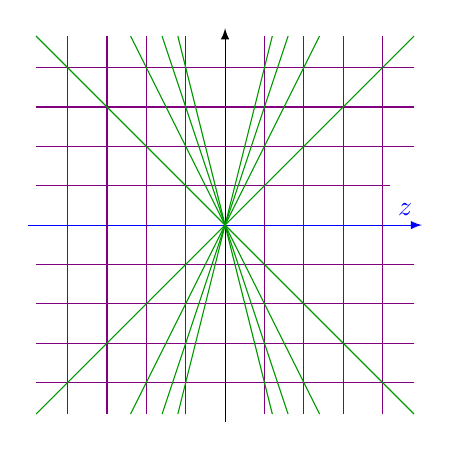
\begin{tikzpicture}[scale=0.5,>=latex]
  \draw[blue,->] (-5,0) -- (5,0) node[anchor=south east] {$z$};
  \draw[->] (0,-5) -- (0,5);
  \draw[violet] (-4,-4.8) -- (-4,4.8);
  \draw[violet] (-3,-4.8) -- (-3,4.8);
  \draw[violet] (-2,-4.8) -- (-2,4.8);
  \draw[violet] (-1,-4.8) -- (-1,4.8);
  \draw[violet] (1,-4.8) -- (1,4.8);
  \draw[violet] (2,-4.8) -- (2,4.8);
  \draw[violet] (3,-4.8) -- (3,4.8);
  \draw[violet] (4,-4.8) -- (4,4.8);
  \draw[violet] (-4.8,1) -- (4.2,1);
  \draw[violet] (-4.8,-1) -- (4.8,-1);
  \draw[violet] (-4.8,2) -- (4.8,2);
  \draw[violet] (-4.8,-2) -- (4.8,-2);
  \draw[violet] (-4.8,3) -- (4.8,3);
  \draw[violet] (-4.8,-3) -- (4.8,-3);
  \draw[violet] (-4.8,4) -- (4.8,4);
  \draw[violet] (-4.8,-4) -- (4.8,-4);
  \draw[green!60!black] (-4.8000,-4.8) -- (4.8000,4.8);
  \draw[green!60!black] (-4.8000,4.8) -- (4.8000,-4.8);
  \draw[green!60!black] (-2.4000,-4.8) -- (2.4000,4.8);
  \draw[green!60!black] (-2.4000,4.8) -- (2.4000,-4.8);
  \draw[green!60!black] (-1.6000,-4.8) -- (1.6000,4.8);
  \draw[green!60!black] (-1.6000,4.8) -- (1.6000,-4.8);
  \draw[green!60!black] (-1.2000,-4.8) -- (1.2000,4.8);
  \draw[green!60!black] (-1.2000,4.8) -- (1.2000,-4.8);
\end{tikzpicture}
\end{document}
